\documentclass[10pt,letterpaper]{article}
\usepackage[top=0.85in,left=2.75in,footskip=0.75in]{geometry}
\usepackage{graphicx}
\usepackage[draft]{hyperref}
\usepackage[font=bf]{caption}


% Text layout specific to Supplemental Materials
\topmargin 0.0cm
\oddsidemargin 0.5cm
\evensidemargin 0.5cm
\textwidth 16cm
\textheight 21cm

\setlength{\parskip}{1em}

\pagestyle{empty} %%in order to delete the number at the bottom of the page


\begin{document}
\section*{Supplementary Figures}
\newpage

\begin{figure*}[h!]
\centering
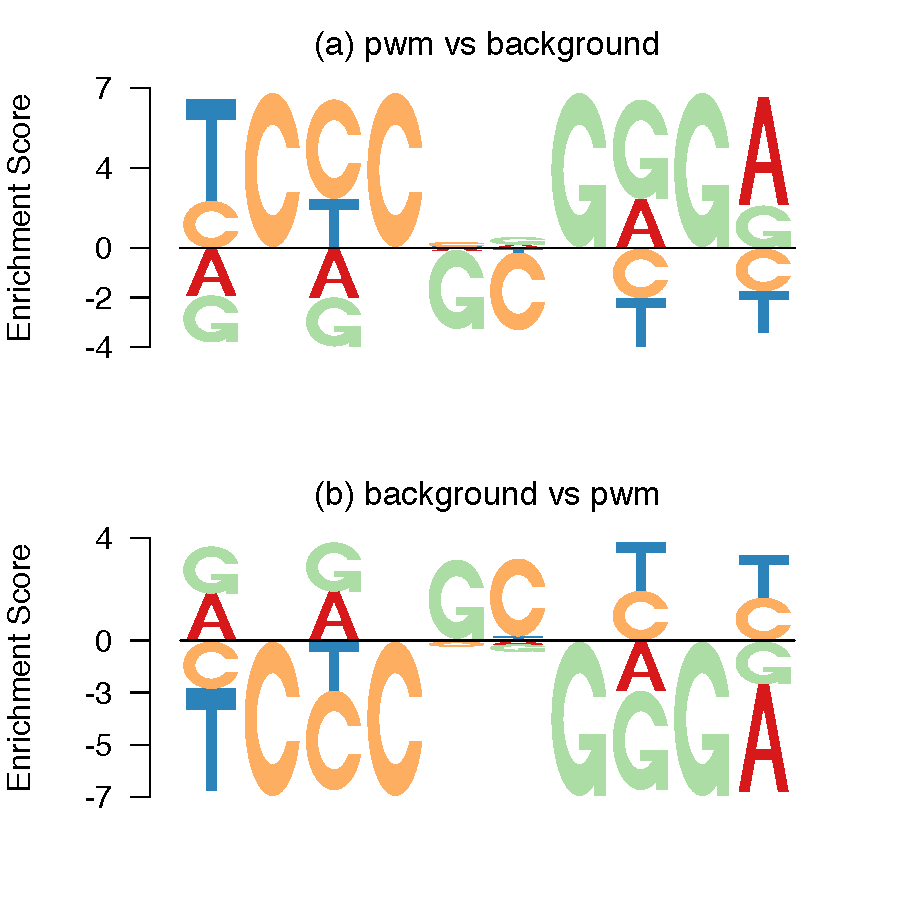
\includegraphics[height=5in, width=5in]{../figures/Figure8.pdf}
\caption{\textbf{Mirror Property of EDLogo}: (panel a) EDLogo plot of the  position weight matrix (PWM) of the primary discovered motif \textit{disc1} (in ENCODE \cite{Kheradpour2013}) of the EBF1 transcription factor against uniform background. (panel b) EDLogo plot of a uniform PWM against the PWM of  EBF1 \textit{disc1} motif as background. The figure demonstrates the fact that, under the scoring scheme in Equation 1, the \textit{EDLogo} plot of a position weight vector $p$ with respect to a background weight vector $q$ is the exact mirror image of the \textit{EDLogo} plot of $q$ against $p$ as background.}
\label{fig:suppfig1}
\end{figure*}


\begin{figure*}[h!]
\centering
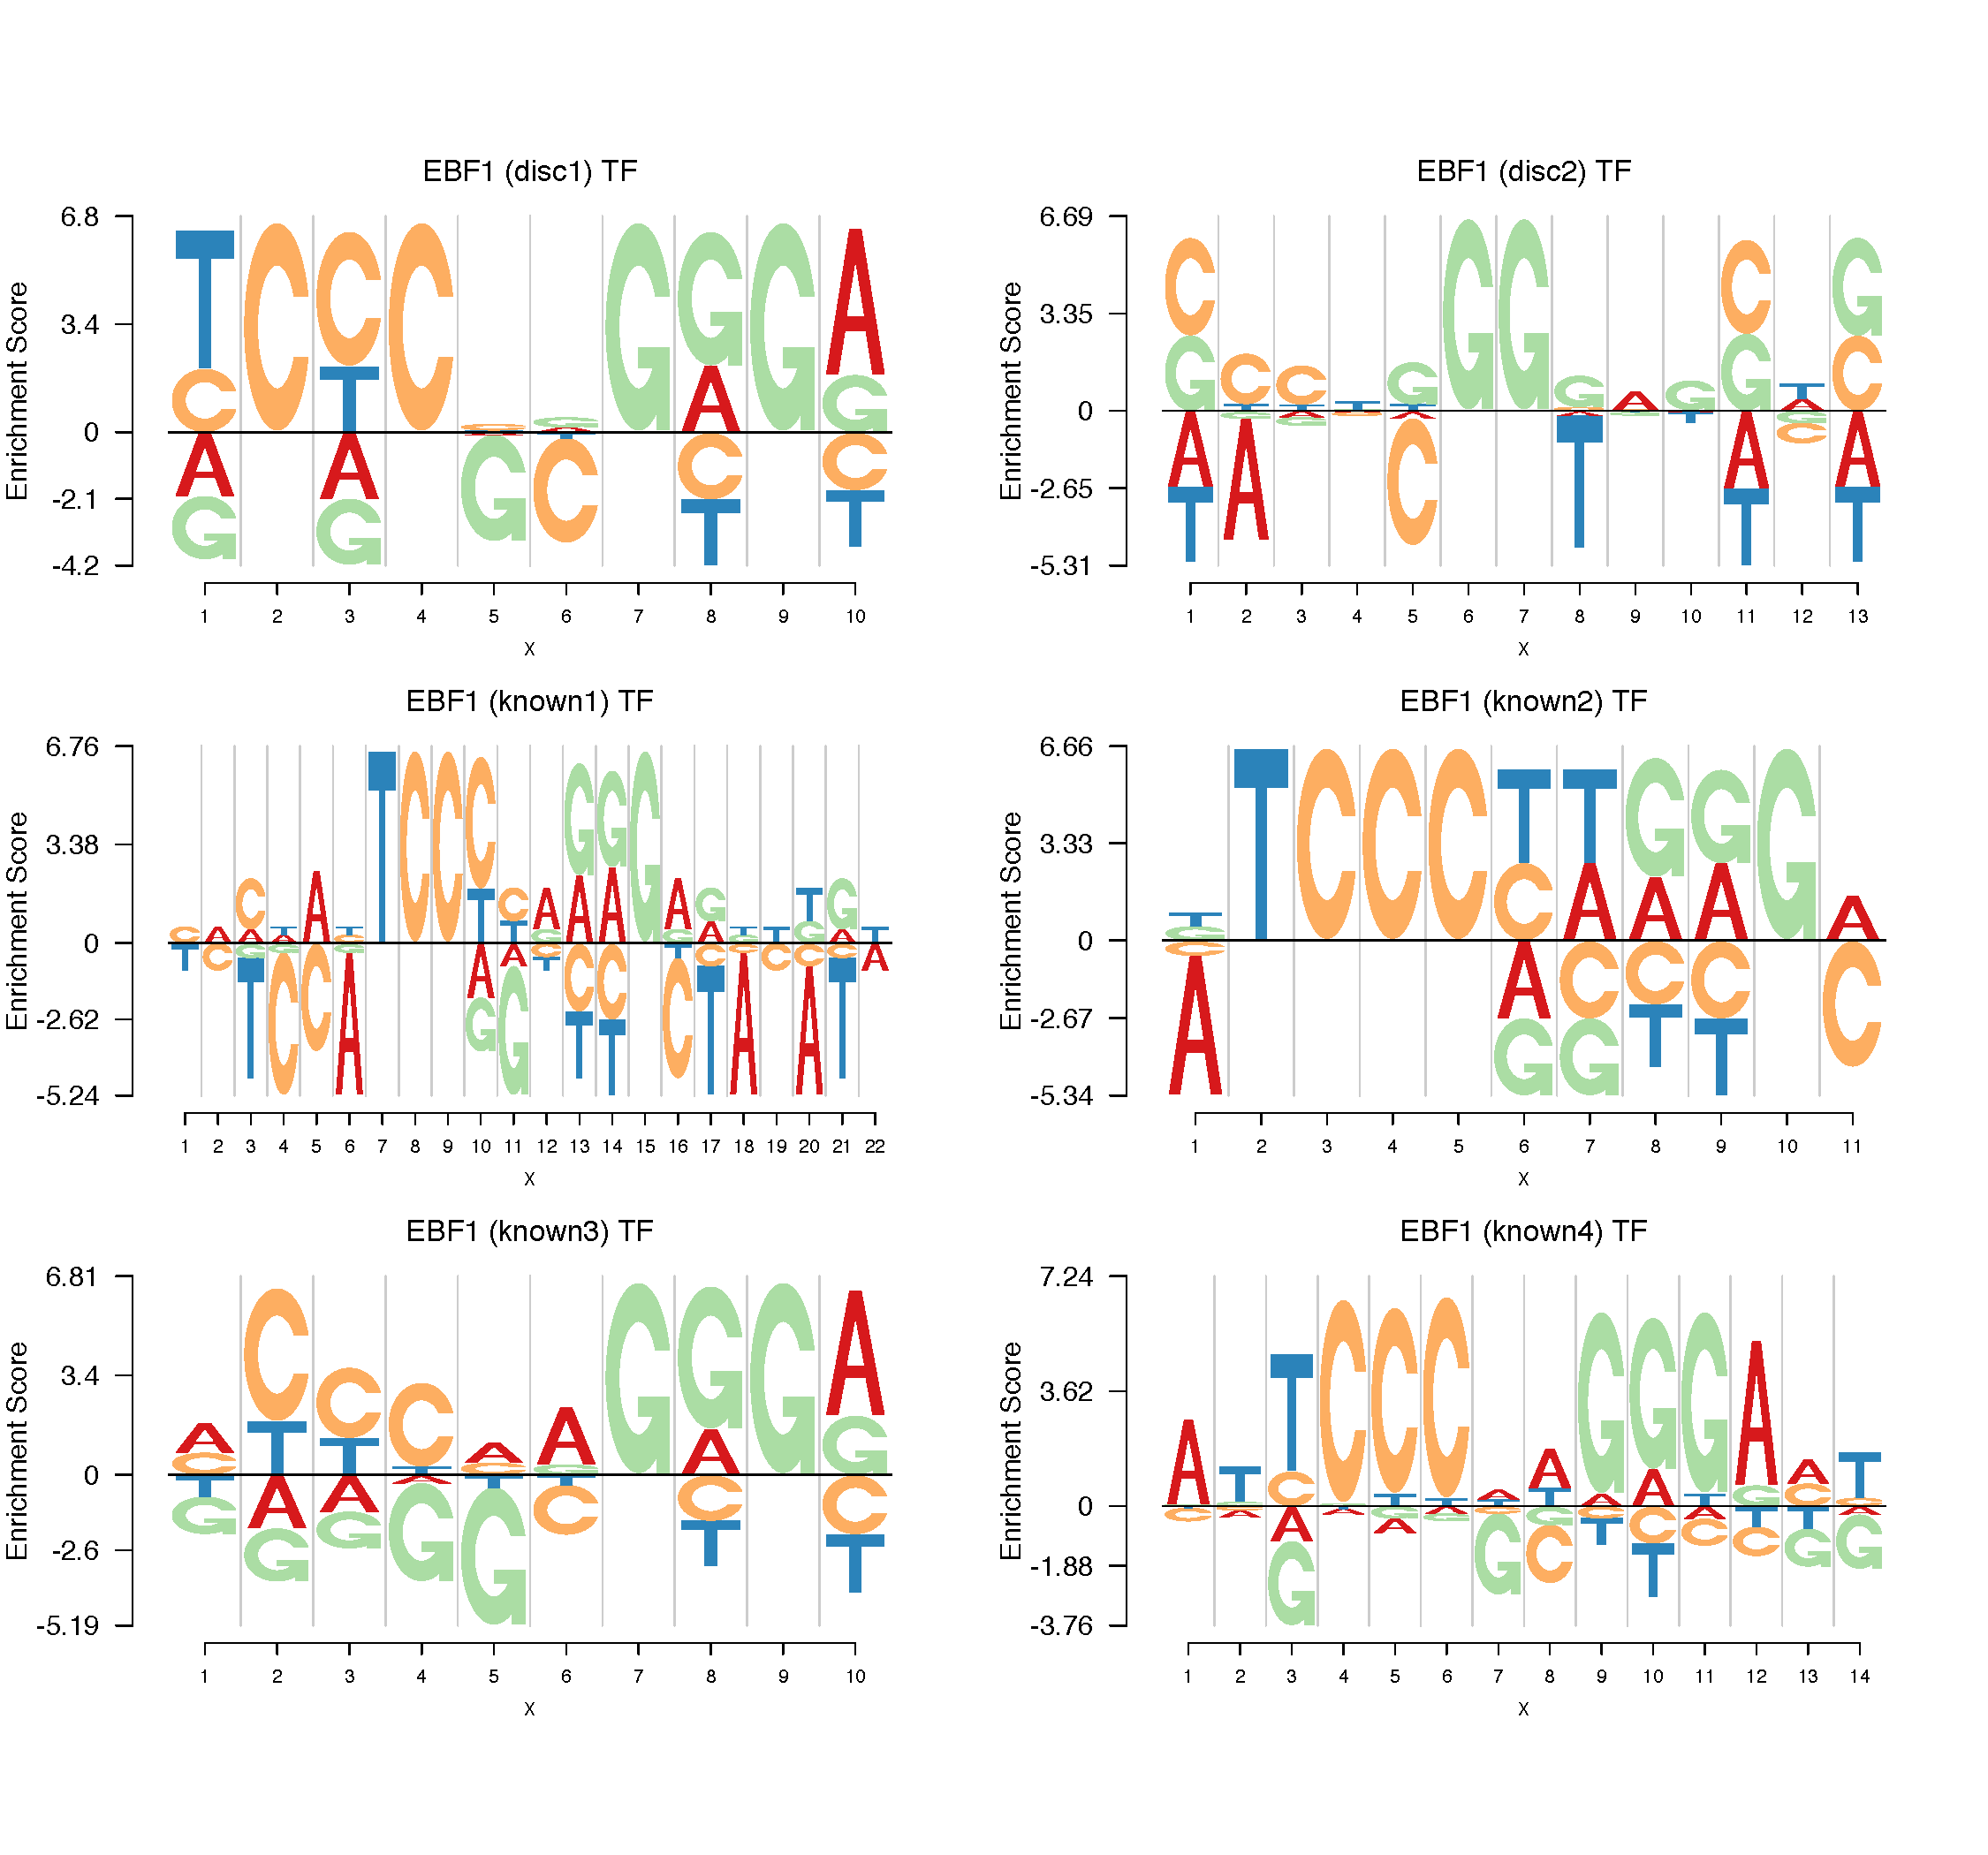
\includegraphics[height=6in, width=7in]{../figures/Figure2.pdf}
\caption{\textbf{EDlogo plot of the different motifs of the EBF1 transcription factor}:  \textit{EDlogo} plot is presented for 6 reported motifs of the transcription factor Early B cell Factor 1 (EBF1) in ENCODE project - 4 of which are previously known from literature (\textit{known1} and \textit{known2} from TRANSFAC database \cite{Wingender2000}, \textit{known3} from  JASPAR database \cite{Sandelin2004} and \textit{known4} from \cite{Jolma2013}) and 2 are discovered (\textit{disc1} and \textit{disc2}) by the ENCODE project \cite{Kheradpour2013}.  Two of the known EBF1 motifs (\textit{known3} and \textit{known4}), along with the primary discovered motif \textit{disc1},  showed depletion of G and C in the middle of the binding site.}
\label{fig:suppfig2}
\end{figure*}

\begin{figure*}[h!]
\centering
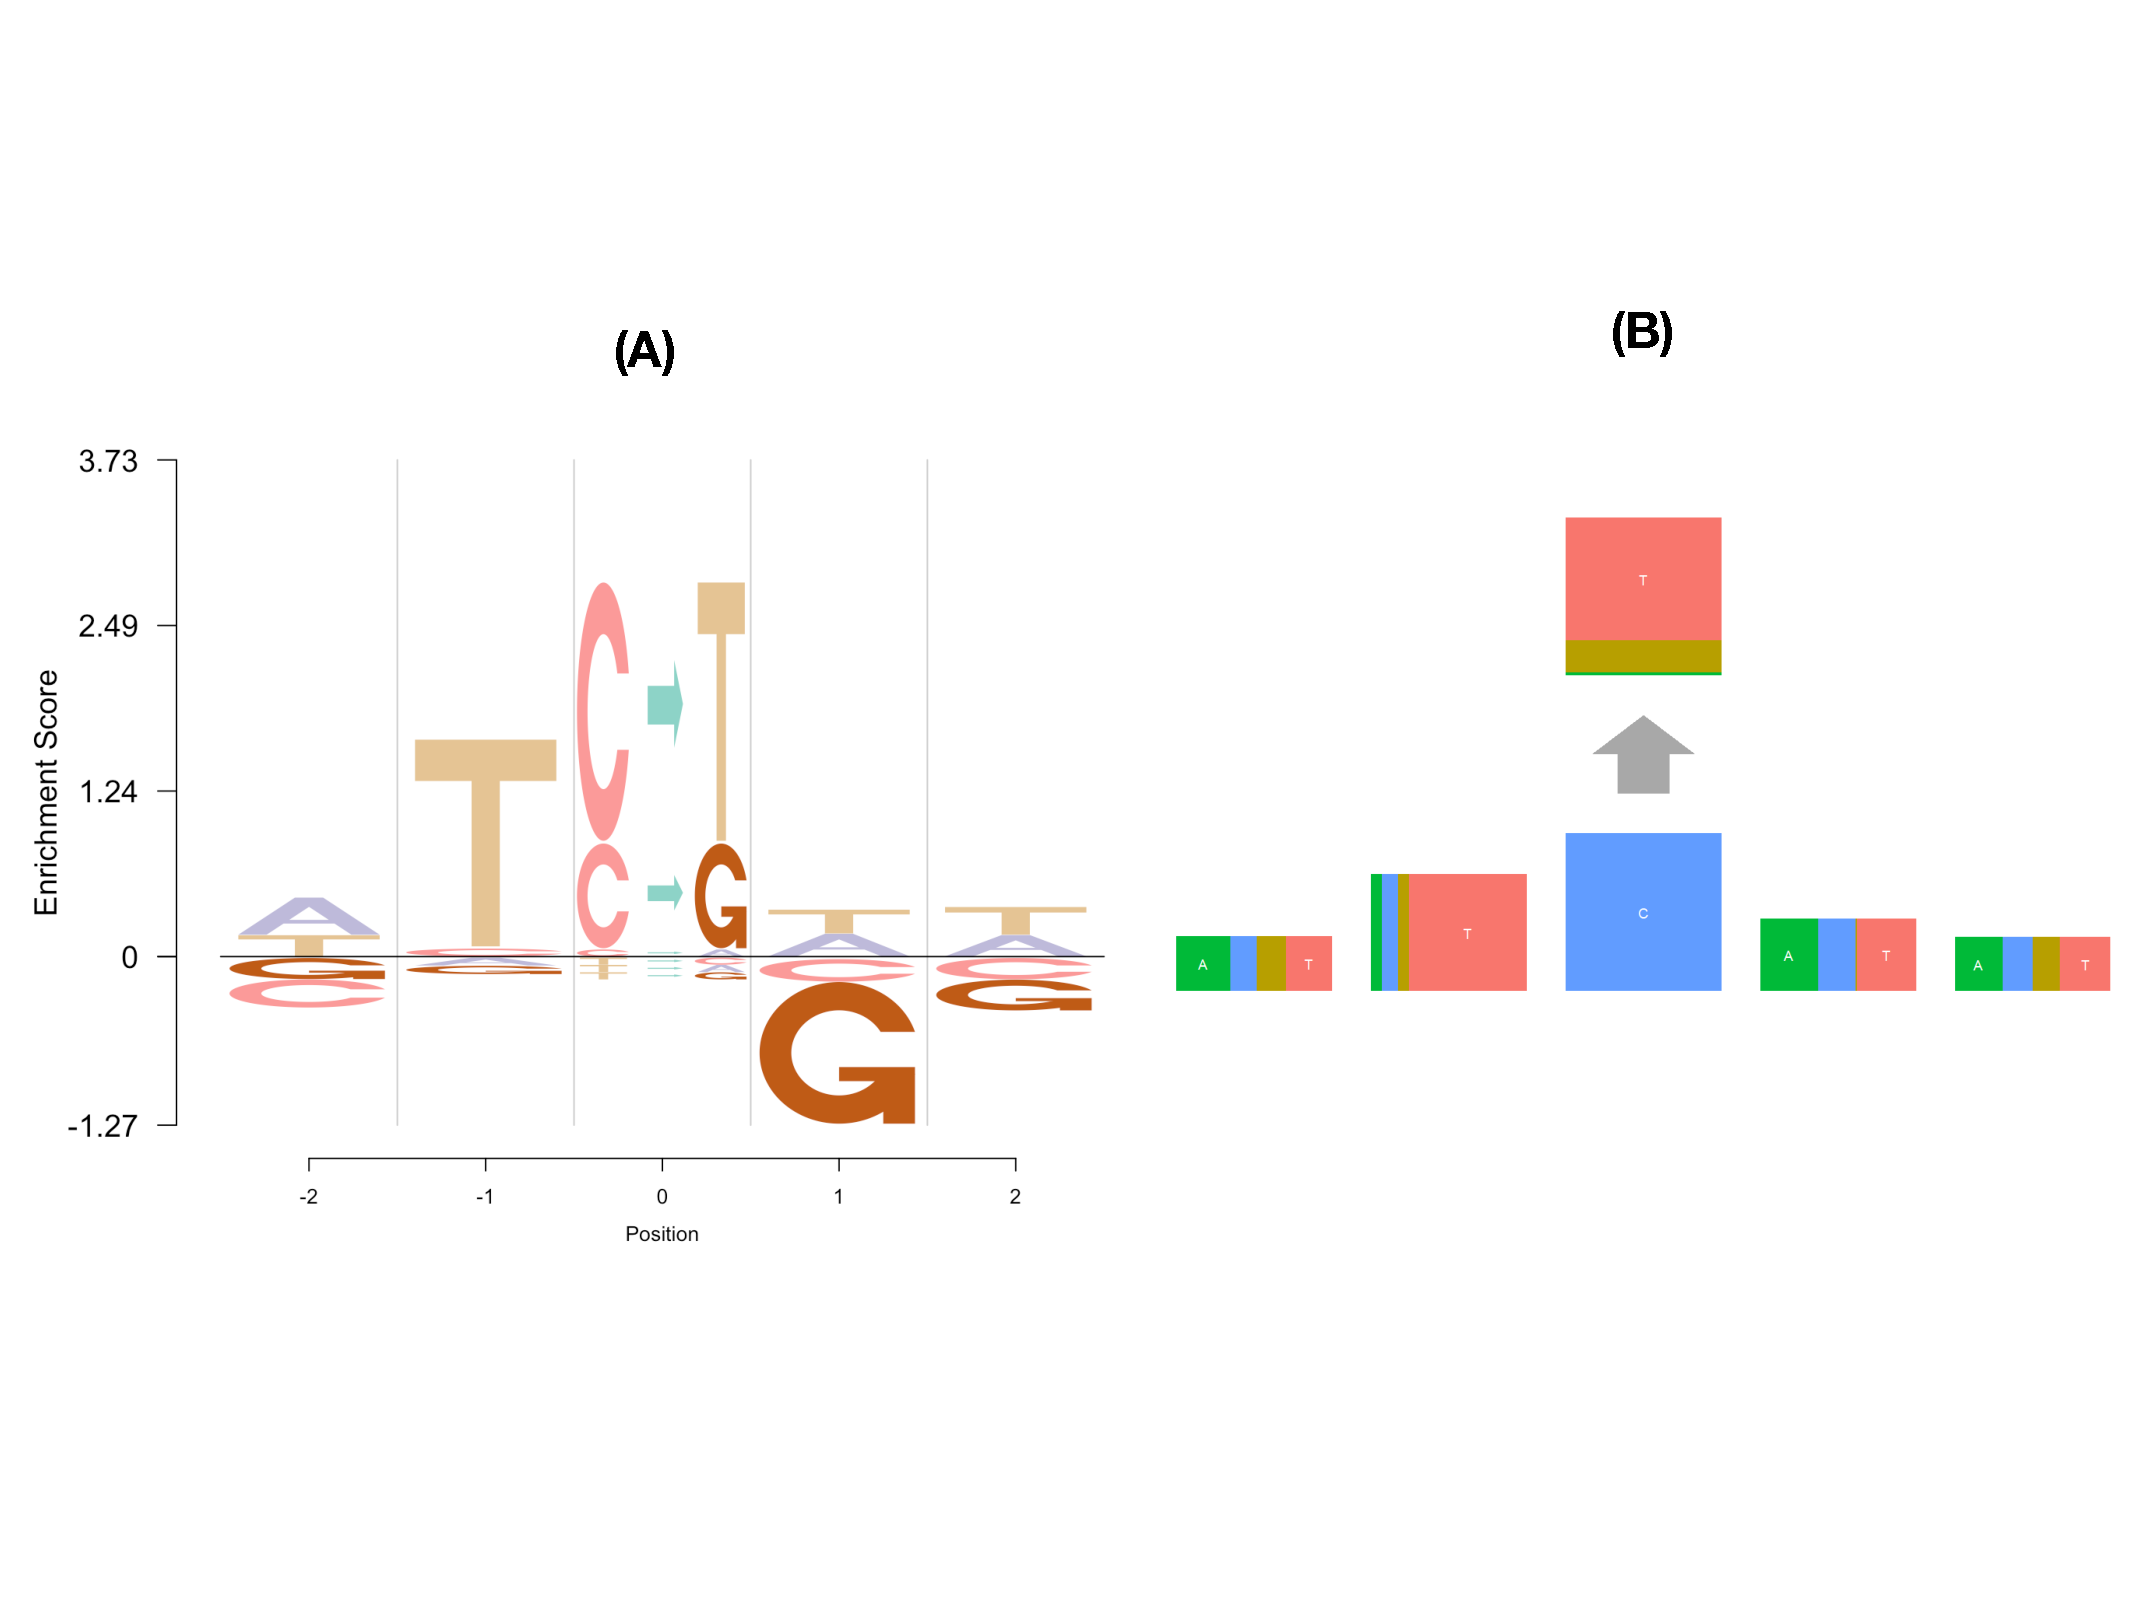
\includegraphics[height=6in, width=7in]{../figures/Figure7/Figure7.pdf}
\caption{\textbf{Comparison of the \textit{EDLogo} plot with pmsignature plot for visualizing cancer mutation signatures}: 
 \textit{EDLogo} plot is compared with the \textit{pmsignature} representation due to Shiraishi et al (2015) \cite{Shiraishi2015} for visualizing the cancer mutation signature of lymphoma B cell \cite{Alexandrov2013}. The \textit{EDLogo} plot shows the depletion of G at the right flanking base more clearly and is arguably more visually appealing in highlighting the overall patterns of the signature compared to the \textit{pmsignature} plot.}
\label{fig:suppfig3}
\end{figure*}



\begin{figure*}[h!]
\centering
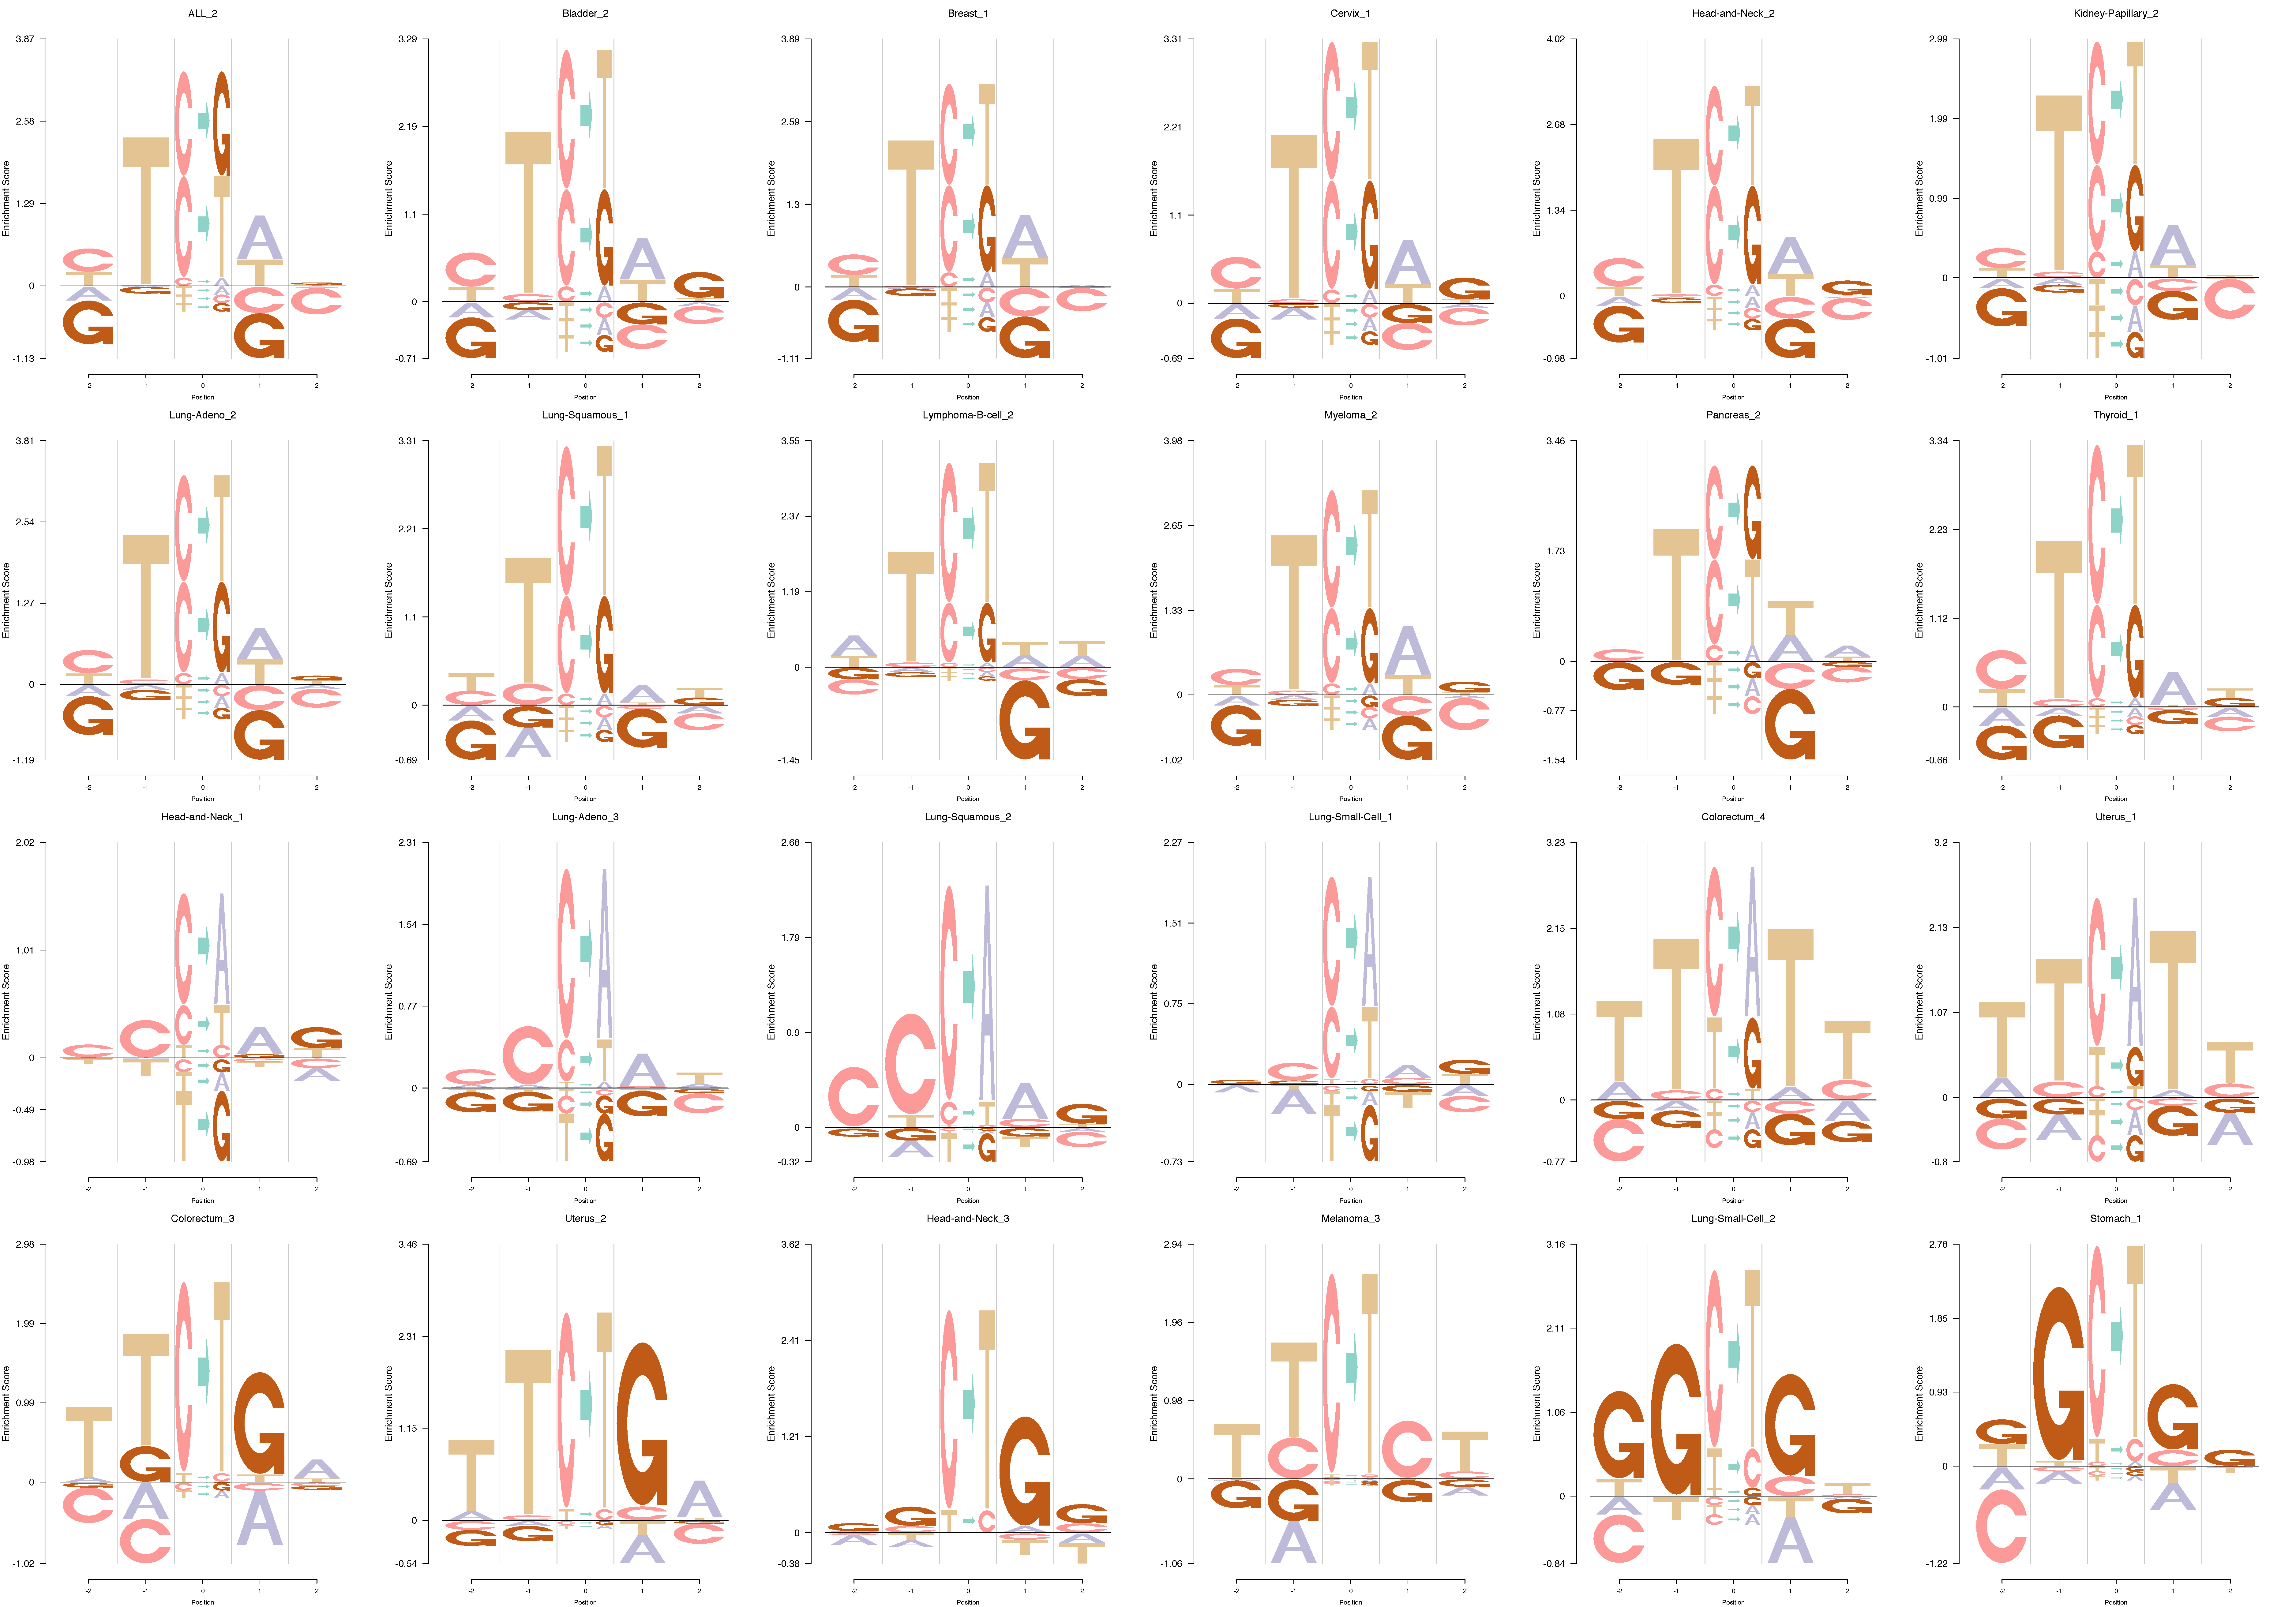
\includegraphics[height=6in, width=7in]{../figures/Figure6.pdf}
\caption{\textbf{EDLogo plots for the mutation signature profiles of different cancer types in Alexandrov et al (2013)}: 
 \textit{EDLogo} plots of the cancer mutational signature profiles for different cancer types collected from across 7042 cancers by Alexandrov et al (2013) \cite{Alexandrov2013}.}
\label{fig:suppfig4}
\end{figure*}


\begin{figure*}[h!]
\centering
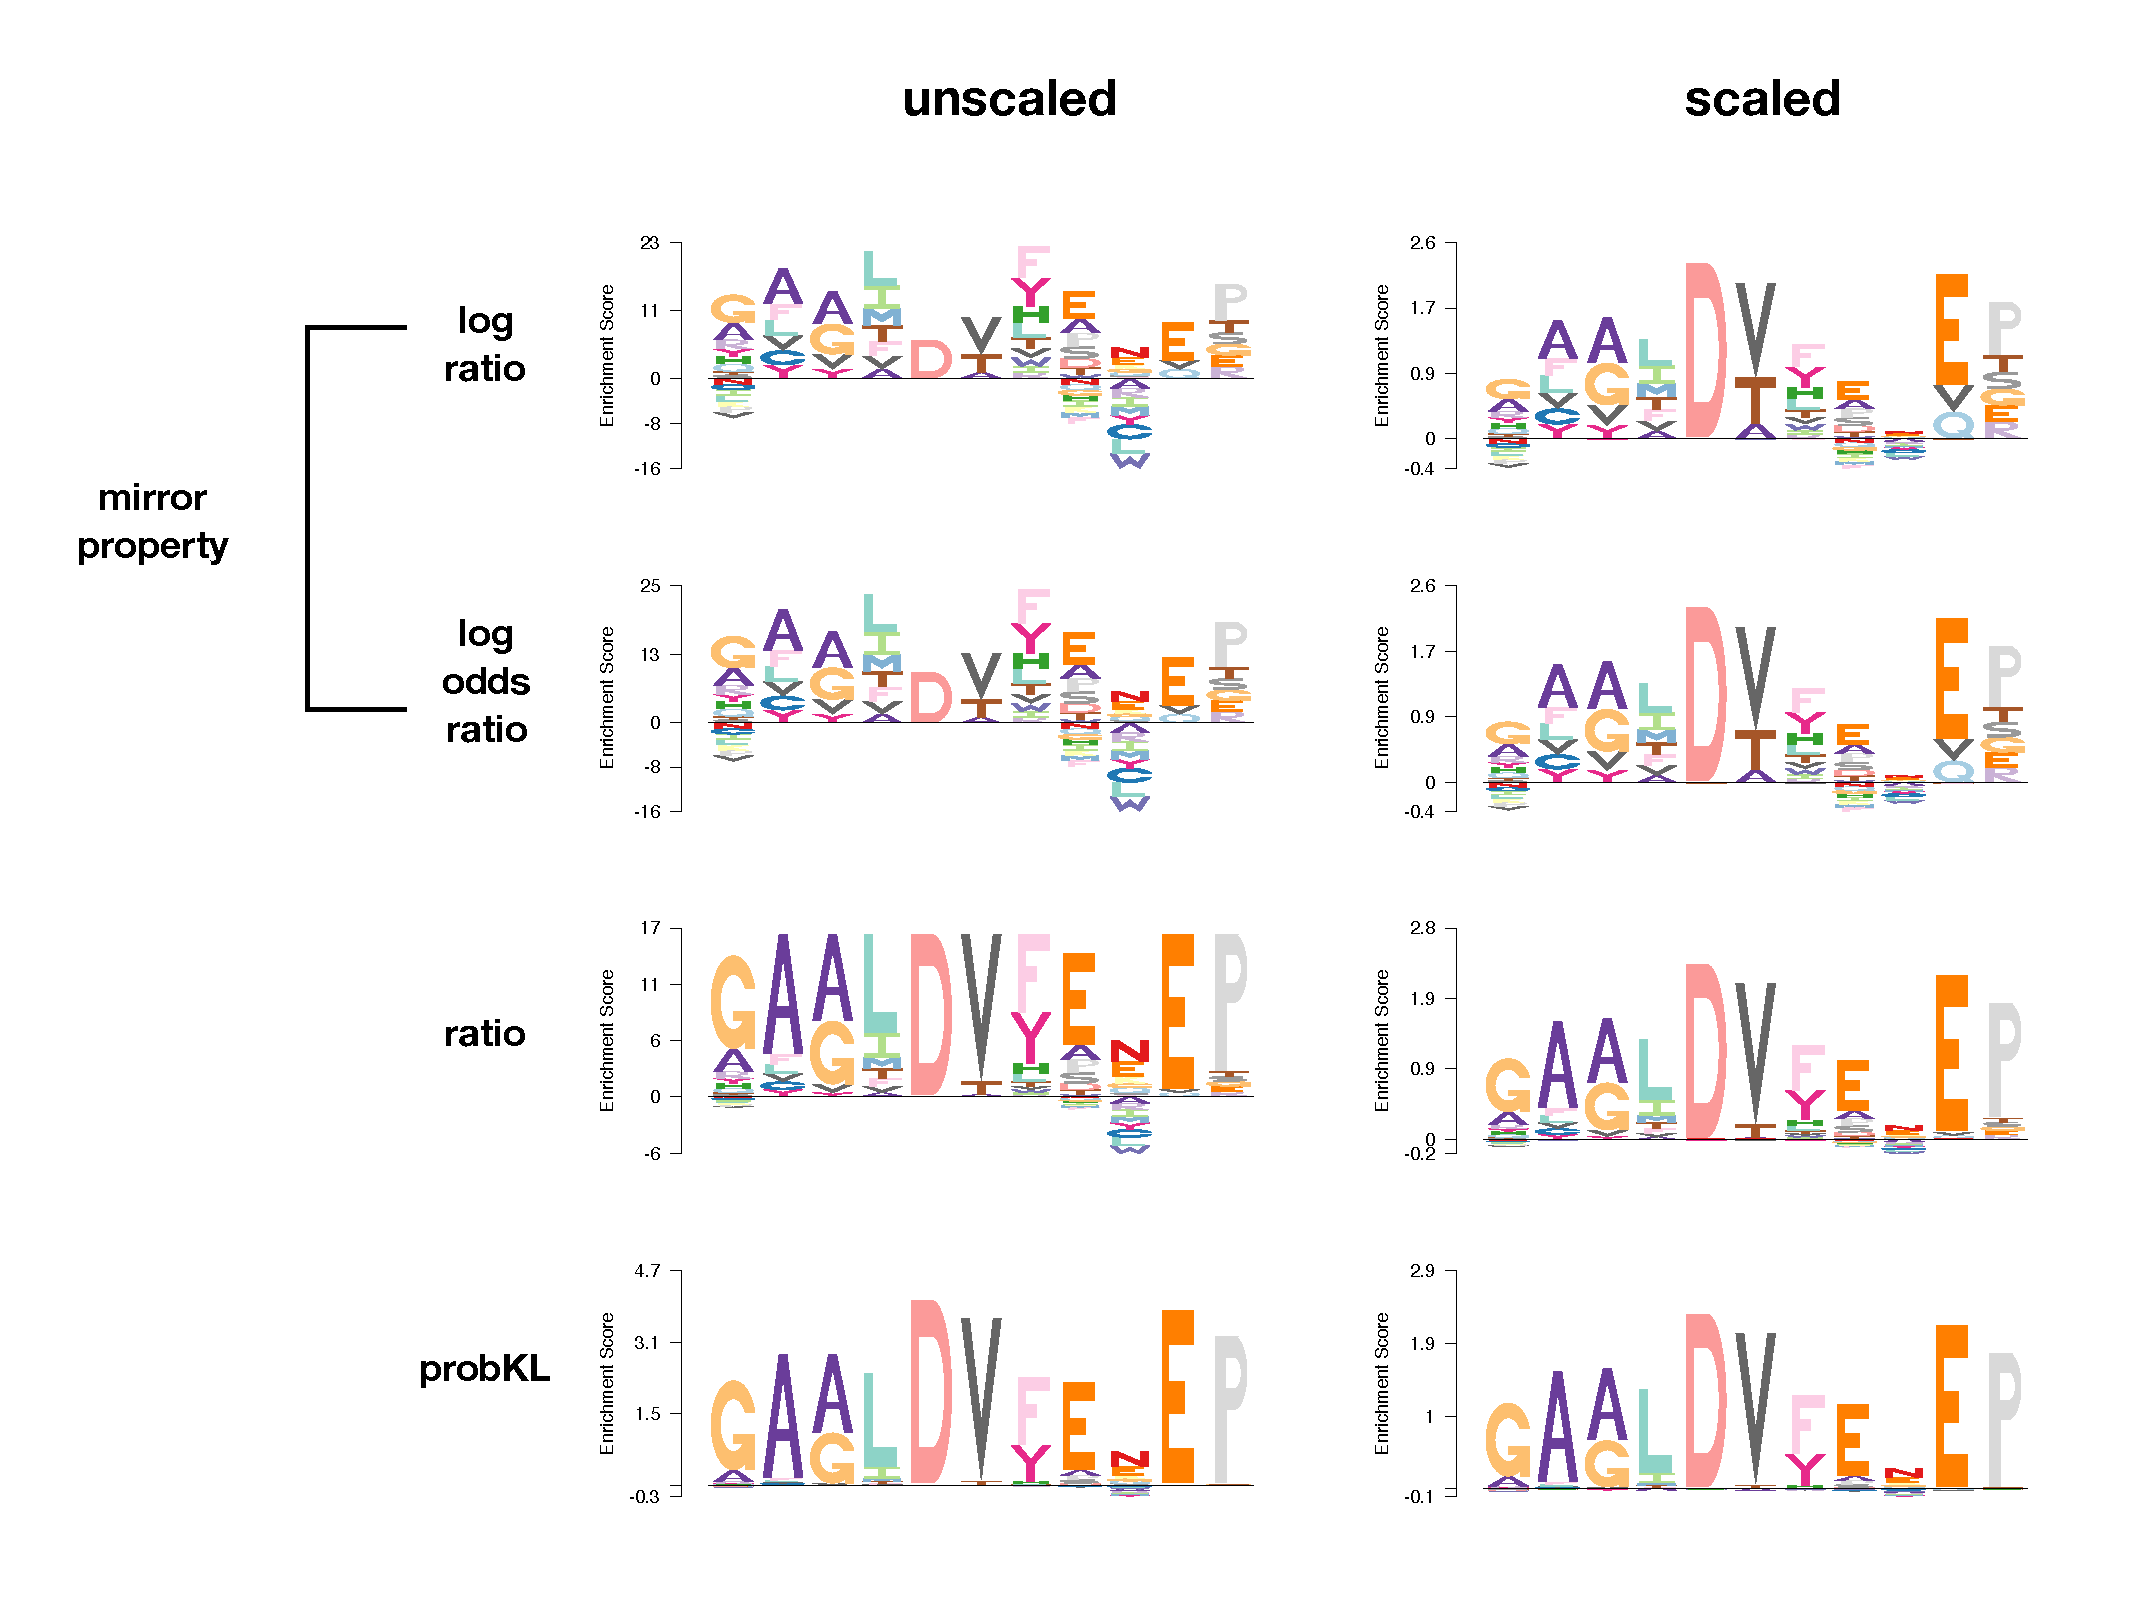
\includegraphics[height=6in, width=7in]{../figures/Figure5/Figure51.pdf}
\caption{\textbf{Different options for EDLogo plot - Protein example}:  \textit{EDLogo} representation  of the binding motif (Motif2 Start=257 Length=11) of the protein \textit{D-isomer specific 2-hydroxyacid dehydrogenase, catalytic domain (IPR006139)} under several other scoring schemes  (\textit{log ratio}, \textit{log odds ratio}, \textit{ratio} and \textit{probKL}) 
with and without the scaling by symmetric Kullback-Leibler divergence against an uniform background.  The \textit{EDLogo} plots for \textit{log ratio} and \textit{log odds ratio} scoring schemes show the ``mirror property'' with or without the scaling.}
\label{fig:suppfig5}
\end{figure*}



\begin{figure*}[h!]
\centering
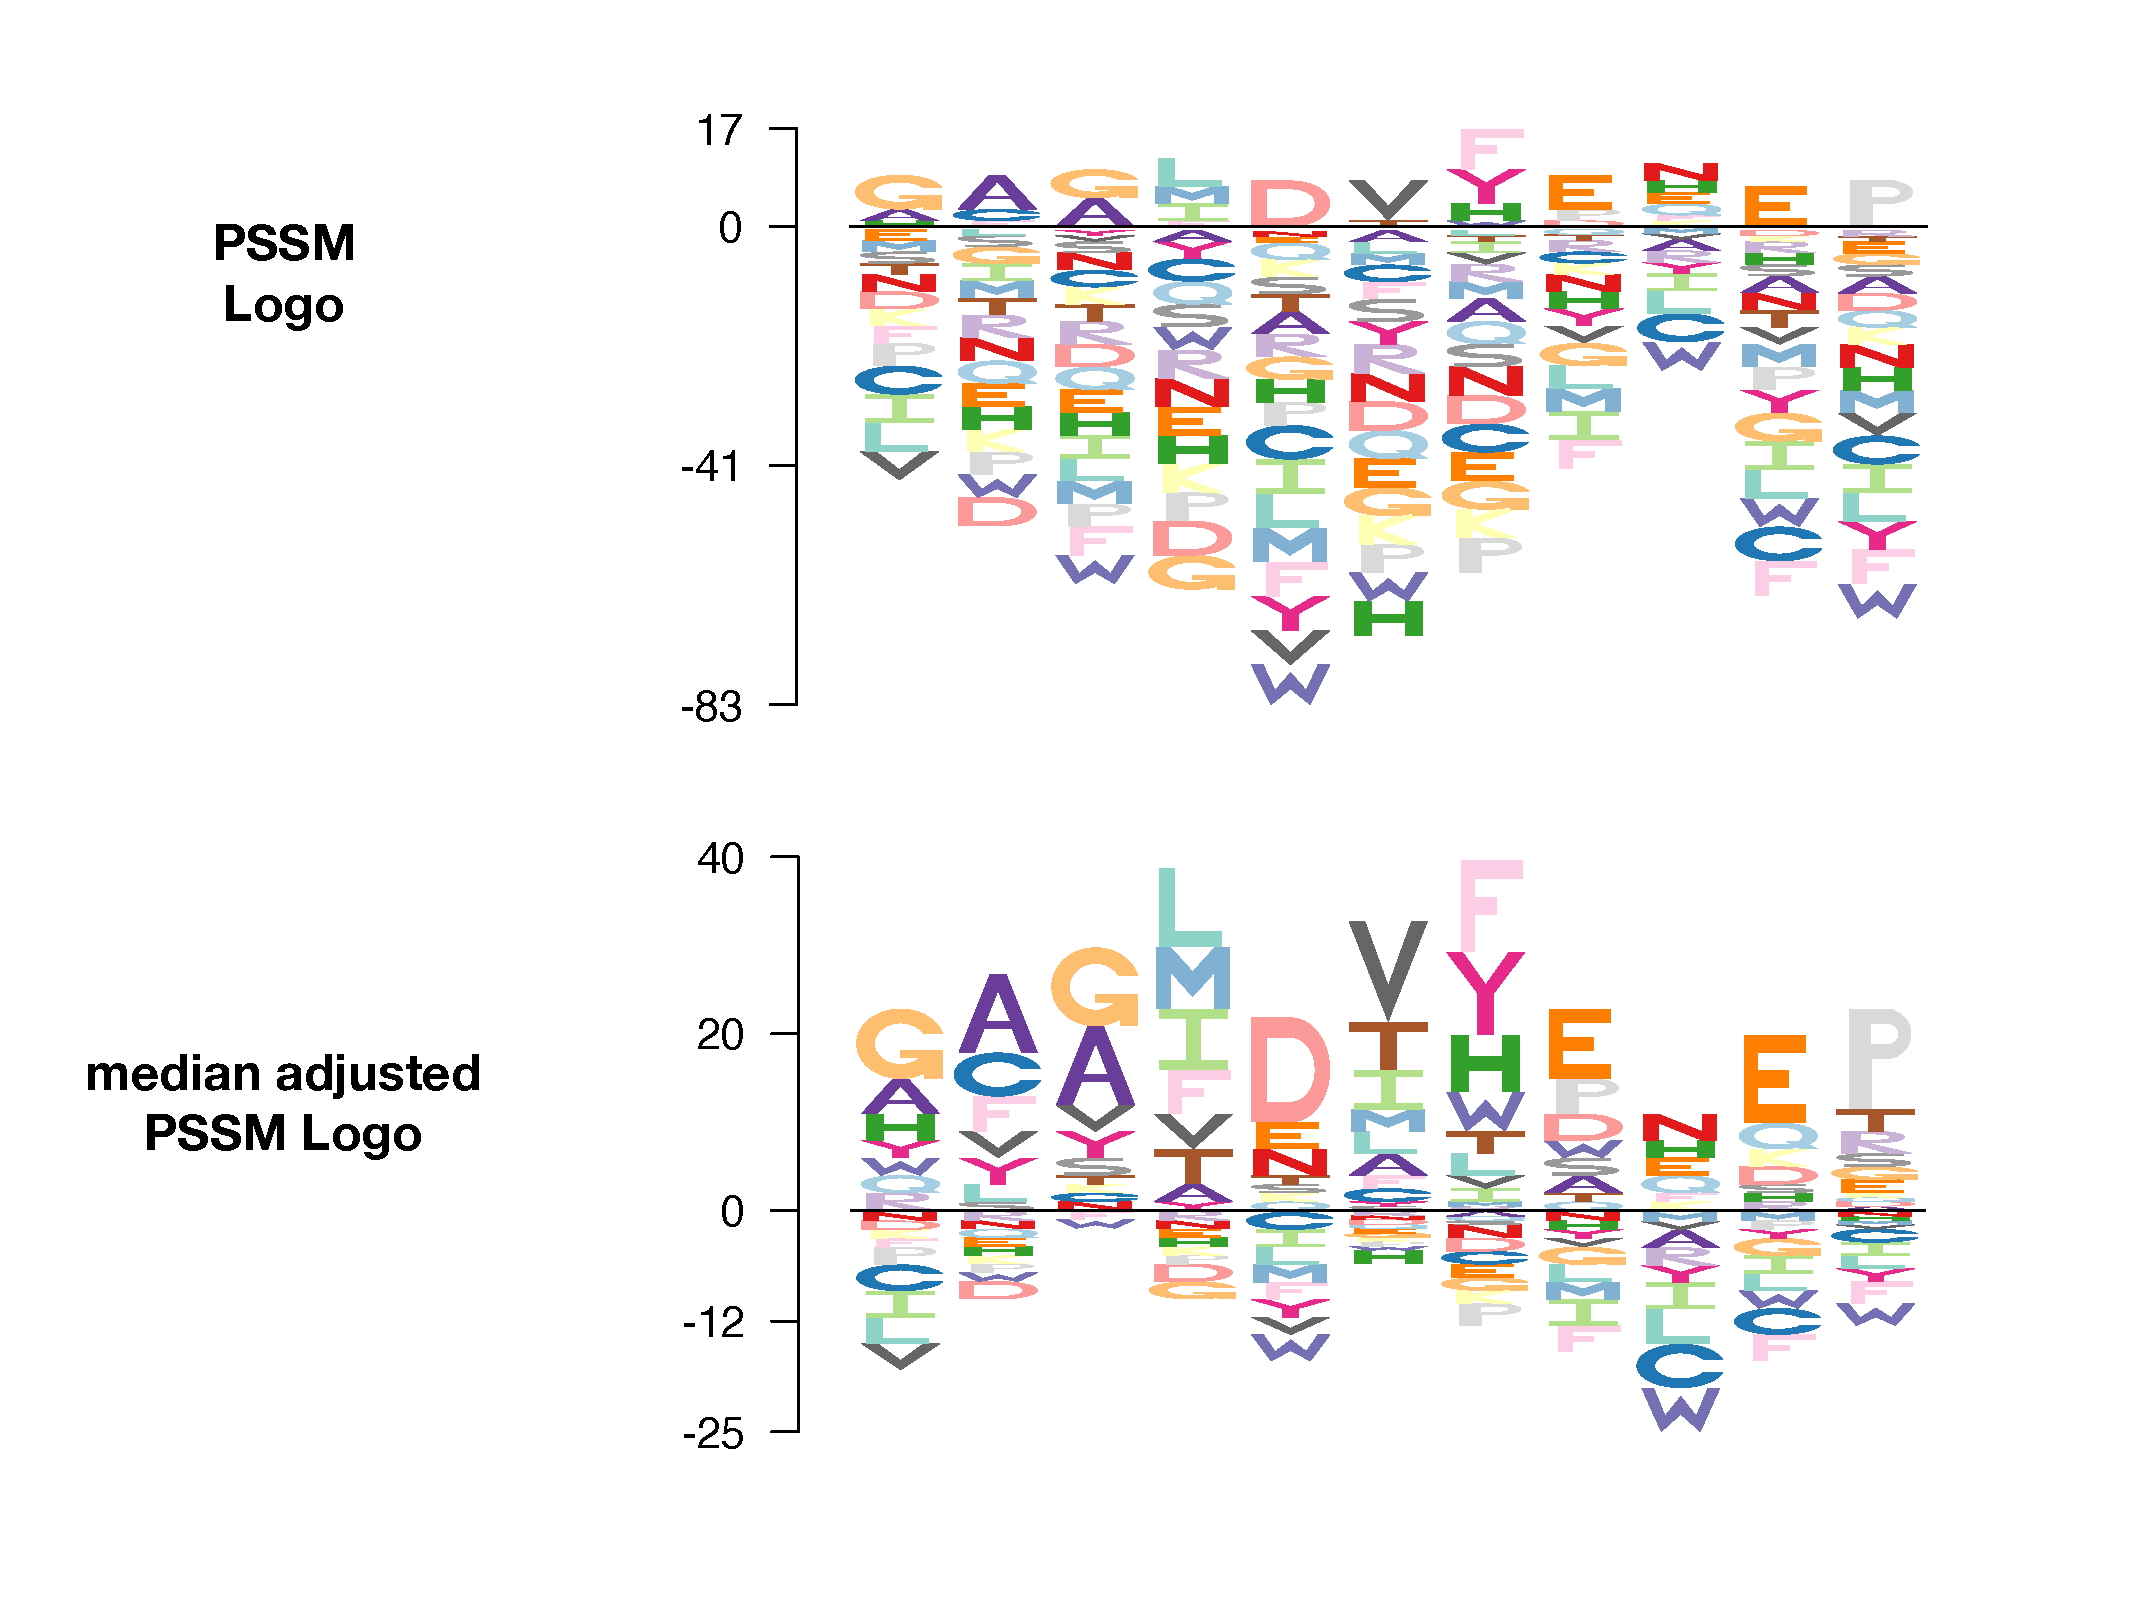
\includegraphics[height=6in, width=7in]{../figures/Figure9/Figure91.pdf}
\caption{\textbf{Logo representation of position specific scoring matrix (PSSM)}: A demonstration of how the median adjustment of position specific scores can reduce visual clutter in logo plot using the example of the binding motif (Motif2 Start=257 Length=11) of the protein \textit{D-isomer specific 2-hydroxyacid dehydrogenase, catalytic domain (IPR006139)}.}
\label{fig:suppfig6}
\end{figure*}

\newpage
\newpage
\newpage
\newpage

\bibliography{bmc_article}      
\bibliographystyle{plainnat}

\end{document}
